\subsection{Árboles generadores y el problema del árbol del generador minimal}

Consideremos el siguiente problema, supongamos que para llevar conexión a internet a un conjunto de ciudades, se quiere determinar la manera más económica de distribuir los cables conociendo el costo de conectar algunos de los pares de ciudades.

\begin{defn}
    Al modelar la red con un grafo $G$ indicando el costo de cada conexión, se obtiene lo que se conoce como un \ul{grafo ponderado} (o con peso). Los lados llevan como etiqueta el costo de la conexión que representan.
\end{defn}

\begin{marginfigure}
    \centering
    \begin{tikzpicture}
        \SetVertexArt
        \SetGraphArtColor{blue!40!black}{black}
        \SetGraphUnit{2}
        \Vertices{circle}{a,b,c,d,e,f}
        \tikzset{LabelStyle/.style =
            {fill=white}}
        \Edge[label=$7$](a)(b)
        \Edge[label=$8$](a)(c)
        \Edge[label=$5$](a)(e)
        \Edge[label=$6$](b)(f)
        \Edge[label=$4$](b)(c)
        \Edge[label=$5$](c)(f)
        \Edge[label=$2$](c)(e)
        \Edge[label=$8$](d)(f)
        \Edge[label=$6$](e)(f)
    \end{tikzpicture}
    \label{fig:ponderado}
    \caption{Ejemplo de grafo ponderado}
\end{marginfigure}

Para este problema lo que queremos es que todas las ciudades estén conectadas (conexidad) y para evitar desperdicios, evitamos los ciclos. Es decir, queremos hallar un árbol como subgrafo de $G$ que tenga todos los vértices y que además represente el costo mínimo de la red. Los pesos de los lados vienen dados por una función $p$, y lo que se quiere es hallar un $T$ que minimice

\[
p(T) = \sum_{l \in T} p(l)
\]

En general, este árbol se define de la siguiente manera:

\begin{defn}
    Suponga que $G = (V, L)$ sea un grafo conexo, y $T$ el subconjunto de $L$ tal que
    
    \begin{itemize}
        \item Cada vértice de $G$ está en un lado de $T$.
        \item Los lados de $T$ forman un árbol.
    \end{itemize}
    
    En este caso, decimos que $T$ es un \ul{árbol generador} de $G$. Para un grafo ponderado, un árbol generador tal que la suma de los pesos de sus lados es mínima, se llama \ul{árbol generador minimal (AGM)}.
\end{defn}

Para resolver este problema, podríamos utilizar un algoritmo voraz: Es decir, partiendo de un vértice $x$, elegimos el lado con menor peso que incide en $x$, digamos $l = xy$, y continua con el lado con menor peos que incide en $y$, si no hay otro lado en $x$ con menor peso. Así sucesivamente hasta agotar los vértices.

\begin{pre}
    ¿El algoritmo voraz nos da un AGM?
\end{pre}

\begin{proof}[Respuesta]
    Supongamos que $G$ es un grafo conexo con $n$ vértices y ponderado con la función $p$. $T$ es un árbol generador de $G$ obtenido con el algoritmo anterior y $U$ es también un árbol generador de $G$.
    
    En primer lugar, enumeremos los lados de $T$ siguiendo el orden del algortimo: $l_1, \dots, l_{n-1}$. Sea $l_k = xy$ el primero de los lados de $T$ que no está en $U$. Llamemos $S$ al conjunto de vértices del subárbol de $T$ que pertenecen a los lados $l_1, \dots, l_{k-1}$. Entonces $x \in S$ e $y \notin S$.
    
    Como $U$ es un árbol generador de $G$, entonces existe un camino en $U$ de $x$ hasta $y$, y un lado $\Bar{l}$ con al menos un vértice $z \in S$ y otro fuera de $S$. Como $\Bar{l}$ no fue elegido por el algoritmo voraz, entonces $p(\Bar{l}) \geq p(l_k)$. Si $\Bar{l}$ está en $T$, tiene que ser algún $e_j$ con $j>k$ por construcción.
    
    Ahora, eliminamos $\Bar{l}$ de $U$ y lo sustituímos por $l_k$ y llamamos al árbol resultante $U_1$. Luego, $U_1$ genera a $T$ y tenemos
    
    \[
    \sum_{l \in L(U_1)} p(l) = \sum_{l \in U} p(l) - p(\Bar{l}) + p(l_k) \leq \sum_{l \in L(U)} p(l)
    \]
    
    Obtuvimos de esta forma un árbol generador con menos peso que $U$ y que tiene el lado $l_k$. Iterando, obtendremos de forma sucesiva los árboles $U_2, \dots, U_m$ (con $m$ siendo la diferencia entre los lados de $U$ y los de $T$), cada uno con menos peso y más lados de $T$.
    
    Eventualmente, obtendremos 
    
    \[
    U_m = T \quad \text{con} \quad \sum_{l \in L(T)} p(l) \leq \sum_{l \in L(U)} p(l)
    \]
    
    \noindent y de esta forma, queda demostrado.
\end{proof}

De esta forma, hemos pasado a demostrar el siguiente teorema:

\begin{teo}
    Si $T$ es un árbol generador de un grafo conexo ponderado $G$ obtenido mediante el algoritmo voraz, entonces $T$ es un AGM para $G$.
\end{teo}